% --- IMPORTS ---
\documentclass[leqno]{article}
\usepackage{graphicx}
\usepackage{dsfont}
\usepackage{mathtools}
\usepackage{amssymb}
\usepackage{amsmath}
\usepackage{amsthm}
\usepackage{float}
\usepackage{ragged2e}
\usepackage{tensor}
\usepackage{fancyhdr}
\usepackage{empheq}
\usepackage[most]{tcolorbox}
\usepackage{enumitem}
\usepackage{dirtytalk}
\usepackage{marginnote}
\usepackage{microtype}
\usepackage[
  a4paper,
  left=0.8in,
  right=1in,
  top=1in,
  bottom=0.5in,
  headheight=14pt,
  headsep=0.4in
]{geometry}
\setlength{\parindent}{0cm}
% --- TikZ Packages ---
\usepackage{pgfplots}
\pgfplotsset{compat=1.18}
\usepgfplotslibrary{fillbetween, polar}
\usetikzlibrary{calc, positioning}
\usetikzlibrary{angles, quotes}
\usetikzlibrary{arrows.meta}
\usetikzlibrary{decorations.pathreplacing, decorations.markings}
\usetikzlibrary{patterns}
\usetikzlibrary{intersections}
% --- URL Packages ---
\usepackage[colorlinks=true,linkcolor=red,citecolor=magenta,urlcolor=black]{hyperref}%
\urlstyle{same}
% --- END OF IMPORTS ---

% --- CUSTOM COMMANDS ---
\RenewDocumentCommand{\marks}{o m}{%
  \IfValueTF{#1}%
    {\marginnote{\raggedright\textbf{[#2]}}[#1]}%
    {\marginnote{\raggedright\textbf{[#2]}}}%
}
\newcommand{\vspacerule}[2]{%
  \par\vspace*{#1}%
  \noindent\hrulefill\par
  \vspace*{#2}%
}
\definecolor{scarlet}{RGB}{205, 40, 75}
\newcommand{\questionitem}{%
  \item\phantomsection
  \addcontentsline{toc}{section}{Question \number\value{enumi}}%
}
\renewcommand{\contentsname}{Questions}
% --- END OF CUSTOM COMMANDS ---

% --- HEADER CONFIG ---
\pagestyle{fancy}
\fancyhead{}
\fancyfoot{}
\renewcommand{\headrulewidth}{0.9pt}
\lhead{Integration of Polar Curves}
\chead{}
\rhead{\href{https://danieljsmith.org}{danieljsmith.org}}
% --- END OF HEADER CONFIG ---

\begin{document}
\vspace*{20pt}
\tableofcontents
\newpage
\begin{enumerate}[
  label=\textbf{\arabic*.},
  leftmargin=*,
  topsep=0pt,
  partopsep=0pt,
  parsep=0pt
]

% ---- Question 1 ----
\questionitem
% [Source: _QBT__Integration_of_Polar_Curves, Q1]

\begin{figure}[H]
    \centering
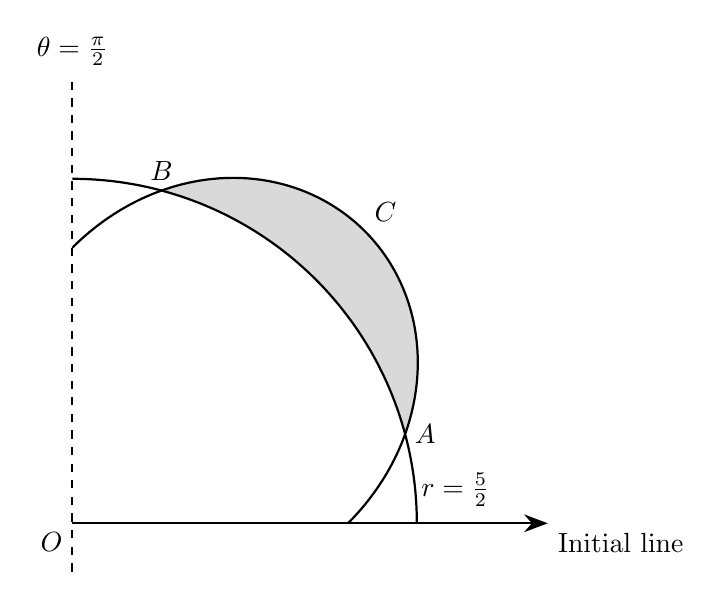
\begin{tikzpicture}[scale=1.75]
\def\R{2.5}
\def\thA{15}
\def\thB{75}

\coordinate (O) at (0,0);
\coordinate (A) at (\thA:\R);
\coordinate (B) at (\thB:\R);
\coordinate (Clab) at ({(2+sin(2*45))*cos(45)},{(2+sin(2*45))*sin(45)});
\coordinate (Dlab) at ({1*\R*cos(10)},{1.*\R*sin(10)});

\draw[dashed, thick] (0,-0.35) -- (0,3.25);
\node[above] at (0,3.25) {$\theta=\frac{\pi}{2}$};

\draw[-{Stealth[length=3mm]}, thick] (0,0) -- (3.45,0) node[below right] {Initial line};

\fill[gray!30]
  plot[smooth, samples=140, domain=\thA:\thB]
    ({(2+sin(2*\x))*cos(\x)},{(2+sin(2*\x))*sin(\x)})
  --
  plot[smooth, samples=140, domain=\thB:\thA]
    ({\R*cos(\x)},{\R*sin(\x)})
  -- cycle;

\draw[thick]
  plot[smooth, samples=160, domain=0:90]
    ({\R*cos(\x)},{\R*sin(\x)});

\draw[thick]
  plot[smooth, samples=220, domain=0:90]
    ({(2+sin(2*\x))*cos(\x)},{(2+sin(2*\x))*sin(\x)});

\node[below left] at (O) {$O$};
\node[right] at (A) {$A$};
\node[above] at (B) {$B$};
\node[above right] at (Clab) {$C$};
\node[below right] at (Dlab) {$r=\frac{5}{2}$};
\end{tikzpicture}
\end{figure}


The diagram shows part of the curve $C$ with polar equation
\[
r=2+\sin 2\theta,\quad 0\leq\theta\leq\frac{\pi}{2}
\] \\
and the circle
\[
r=\frac{5}{2}
\] \\
The curve and the circle intersect at the points $A$ and $B$, as shown. \\

Find, correct to three significant figures, the area of the shaded region enclosed by $C$ and the circle. \marks{9} \\

\newpage


% ---- Question 2 ----
\questionitem
% [Source: _QBT__Integration_of_Polar_Curves, Q2]

\begin{enumerate}[label=\textbf{(\alph*)}]
  \item A curve has polar equation $r=a\sin^23\theta$, where $a>0$ and $0\leq \theta<2\pi$. \\
  \begin{enumerate}[label=(\roman*)]
    \item Sketch the curve. \marks{2} \\
    \item Find, in exact form, the total area of the regions enclosed by the curve. \marks{7} \\
  \end{enumerate}
\end{enumerate}
\newpage
% ---- Question 3 ----
\questionitem
% [Source: _QBT__Integration_of_Polar_Curves, Q3]

\begin{figure}[H]
    \centering
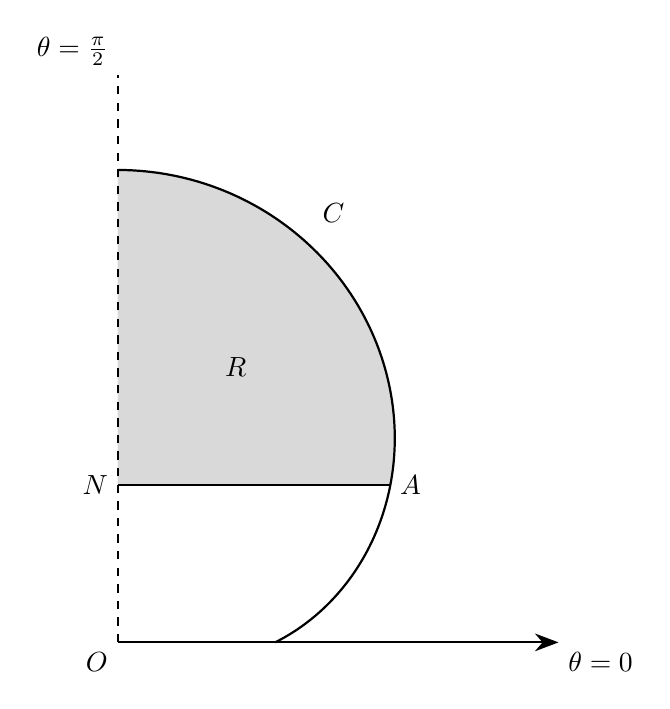
\begin{tikzpicture}[scale=2]
\def\thmax{1.570796}
\def\thA{0.523599}

\coordinate (O) at (0,0);
\coordinate (X) at (2.8,0);
\coordinate (V) at (0,3.6);
\coordinate (A) at (30:2);
\coordinate (N) at ($(O)!(A)!(V)$);
\coordinate (P) at (90:3);

\fill[gray!30] (N) -- (P) --
  plot[smooth, samples=150, domain=\thmax:\thA]
    ({(1+2*sin(deg(\x)))*cos(deg(\x))},{(1+2*sin(deg(\x)))*sin(deg(\x))})
  -- cycle;

\draw[-{Stealth[length=3mm]}, thick] (O) -- (X);
\draw[dashed, thick] (O) -- (V);

\draw[thick]
  plot[smooth, samples=200, domain=0:\thmax]
    ({(1+2*sin(deg(\x)))*cos(deg(\x))},{(1+2*sin(deg(\x)))*sin(deg(\x))});

\draw[thick] (A) -- (N);

\node[below left] at (O) {$O$};
\node[right] at (A) {$A$};
\node[left] at (N) {$N$};
\node[above left] at ({1.1*(1+2*sin(60))*cos(60)},{1.1*(1+2*sin(60))*sin(60)}) {$C$};
\node at (0.75,1.75) {$R$};
\node[above left] at (V) {$\theta=\frac{\pi}{2}$};
\node[below right] at (X) {$\theta=0$};
\end{tikzpicture}
\end{figure}


The curve $C$ shown in the diagram above has polar equation
\[
r=1+2\sin\theta,\quad 0\leq\theta\leq\frac{\pi}{2}
\] \\
The point $A$ on $C$ has $y$-coordinate $1$. \\

The point $N$ lies on the line $\theta=\frac{\pi}{2}$ and $AN$ is perpendicular to the line $\theta=\frac{\pi}{2}$. \\

The finite region $R$, shown shaded in the diagram above, is bounded by the curve $C$, the line $\theta=\frac{\pi}{2}$ and the line $AN$. \\

Find the exact area of the shaded region $R$. \marks{9} \\

\newpage

% ---- Question 4 ----
\questionitem
% [Source: _QBT__Integration_of_Polar_Curves, Q4]

The curve $C$ has polar equation
\[
r^2=\frac{\pi^2-(\theta-\pi)^2}{1+(\theta-\pi)^2}\qquad 0\leq\theta\leq2\pi
\] \\
\begin{enumerate}[label=\textbf{(\alph*)}]
  \item Sketch $C$ and state the polar coordinates of the point on $C$ furthest from the pole. \marks{4} \\
  \item Using the substitution $u=\theta-\pi$, or otherwise, find the exact area enclosed by $C$. \marks{6} \\
\end{enumerate}


\newpage

% ---- Question 5 ----
\questionitem
% [Source: _QBT__Integration_of_Polar_Curves, Q5]

\begin{figure}[H]
    \centering
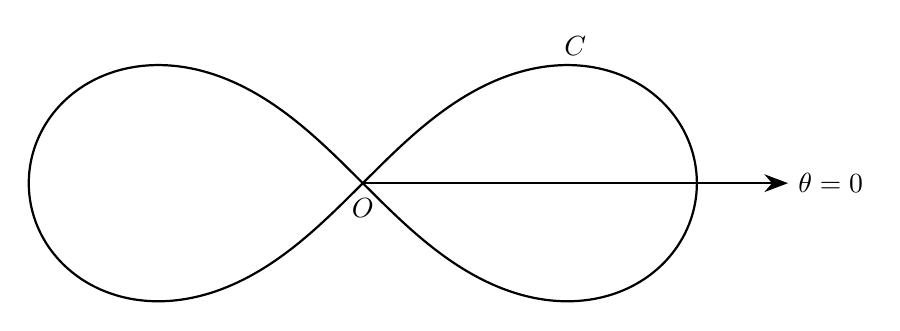
\begin{tikzpicture}[scale=1.5]
\def\K{8}
\def\ArrowLen{3.6}

\coordinate (O) at (0,0);

\draw[-{Stealth[length=3mm]}, thick, black]
  (O) -- (\ArrowLen,0) node[right] {$\theta=0$};

\draw[thick, black]
  (O)
  plot[variable=\t, samples=400, domain=-pi/4:pi/4]
    ({sqrt(max(0,\K*cos(2*\t r)))*cos(\t r)},
     {sqrt(max(0,\K*cos(2*\t r)))*sin(\t r)})
  -- cycle;

\draw[thick, black]
  (O)
  plot[variable=\t, samples=400, domain=3*pi/4:5*pi/4]
    ({sqrt(max(0,\K*cos(2*\t r)))*cos(\t r)},
     {sqrt(max(0,\K*cos(2*\t r)))*sin(\t r)})
  -- cycle;

\node[below, yshift=-2pt] at (O) {$O$};
\node[above right] at
  ({sqrt(\K*cos(2*0.55 r))*cos(0.55 r)},
   {sqrt(\K*cos(2*0.55 r))*sin(0.55 r)})
  {$C$};
\end{tikzpicture}
\end{figure}

\vspace*{10pt}


The diagram below shows the curve $C$ with polar equation $r^2=8\cos 2\theta$. \\

\begin{enumerate}[label=\textbf{(\alph*)}]
  \item Show that a cartesian equation of $C$ is
  \[
  (x^2+y^2)^2=8(x^2-y^2)
  \]
  \marks[-20pt]{4}
  \item Show that the coordinate axes are lines of symmetry of $C$. \marks{2} \\
  \item Find the exact area enclosed by each loop of $C$. \marks{5} \\
\end{enumerate}

\newpage


% ---- Question 6 ----
\questionitem
% [Source: _QBT__Integration_of_Polar_Curves, Q6]

\begin{figure}[H]
    \centering
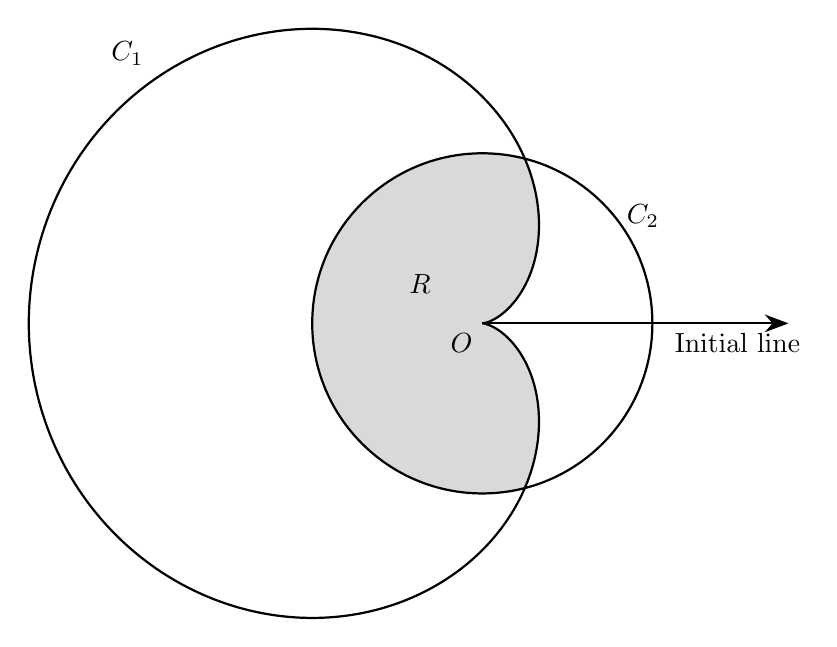
\begin{tikzpicture}[scale=0.9]
\def\aval{1.6}
\def\thA{75.52}
\def\thB{284.48}
\coordinate (O) at (0,0);
\coordinate (COneLabel) at ({2.1*\aval*(1-cos(145))*cos(145)},{2.1*\aval*(1-cos(145))*sin(145)});
\coordinate (CTwoLabel) at (30:1.9*\aval);

\fill[gray!30] (O) --
  plot[smooth, samples=120, domain=0:\thA, variable=\t]
    ({2*\aval*(1-cos(\t))*cos(\t)},{2*\aval*(1-cos(\t))*sin(\t)})
  --
  plot[smooth, samples=180, domain=\thA:\thB, variable=\t]
    ({1.5*\aval*cos(\t)},{1.5*\aval*sin(\t)})
  --
  plot[smooth, samples=120, domain=\thB:360, variable=\t]
    ({2*\aval*(1-cos(\t))*cos(\t)},{2*\aval*(1-cos(\t))*sin(\t)})
  -- cycle;

\draw[thick, black] (O) circle (1.5*\aval);

\draw[thick, black]
  plot[smooth, samples=240, domain=0:360, variable=\t]
    ({2*\aval*(1-cos(\t))*cos(\t)},{2*\aval*(1-cos(\t))*sin(\t)});

\draw[-{Stealth[length=3mm]}, thick, black] (O) -- ({2.7*\aval},0);

\node[below left] at (O) {$O$};
\node[above] at (COneLabel) {$C_1$};
\node[left] at (CTwoLabel) {$C_2$};
\node at ({-0.55*\aval},{0.35*\aval}) {$R$};
\node[below] at ({2.25*\aval},0) {Initial line};
\end{tikzpicture}
\end{figure}


The diagram above shows the curve $C_1$ with polar equation $r=2a(1-\cos\theta)$, $0\leq\theta\leq2\pi$, and the circle $C_2$ with polar equation $r=a$, $0\leq\theta\leq2\pi$, where $a$ is a positive constant. \\
\begin{enumerate}[label=\textbf{(\alph*)}]
  \item Find, in terms of $a$, the polar coordinates of the points where $C_1$ meets $C_2$. \marks{3} \\
\end{enumerate}
The common region enclosed by $C_1$ and $C_2$ is shaded in the diagram above. \\
\begin{enumerate}[label=\textbf{(\alph*)}, resume]
  \item Find the area of the shaded region $R$, giving your answer in the form
  \[
  \frac{1}{12}a^2\left(p\pi+q\sqrt{3}\right)
  \]
  where $p$ and $q$ are integers to be found. \marks{7} \\
\end{enumerate}


\newpage

% ---- Question 7 ----
\questionitem
% [Source: _QBT__Integration_of_Polar_Curves, Q7]

\begin{figure}[H]
    \centering
\begin{tikzpicture}[scale=1.5]
\def\ascl{1}
\coordinate (O) at (0,0);
\coordinate (X) at ({4.6*\ascl},0);
\coordinate (Q) at (45:{4.6*\ascl});
\coordinate (R) at (225:{4.6*\ascl});
\coordinate (A) at (45:{3*\ascl});
\coordinate (B) at ({2*\ascl},0);

\draw[-{Stealth[length=3mm]}, thick] (O) -- (X) node[right] {$\theta=0$};
\draw[dashed] (R) -- (Q);
\pic["$\frac{\pi}{4}$", draw, angle radius=8mm, angle eccentricity=1.35] {angle=X--O--Q};

\draw[thick] (O) circle ({2*\ascl});
\draw[thick, black, samples=400, domain=-180:180, variable=\t]
  plot ({\ascl*(2+sin(2*\t))*cos(\t)},{\ascl*(2+sin(2*\t))*sin(\t)});

\node[below] at (O) {$O$};
\node[right, xshift=3pt] at (A) {$A$};
\node[below right] at (B) {$B$};
\end{tikzpicture}
\end{figure}


The diagram above shows the curve $C$ with polar equation $r=a(2+\sin 2\theta)$ and the circle $r=2a$ for $-\pi\leq\theta\leq\pi$, where $a$ is a positive constant. \\
\begin{enumerate}[label=\textbf{(\alph*)}]
  \item Write down the polar coordinates of the points $A$ and $B$. \marks{2} \\
  \item Explain why $C$ is symmetrical about the line $\theta=\frac{\pi}{4}$. \marks{2} \\
  \item Find, in terms of $a$, the exact total area of the regions that lie inside $C$ and outside the circle. \marks{5} \\
\end{enumerate}


\newpage


% ---- Question 8 ----
\questionitem
% [Source: _QBT__Integration_of_Polar_Curves, Q8]

\begin{figure}[H]
    \centering
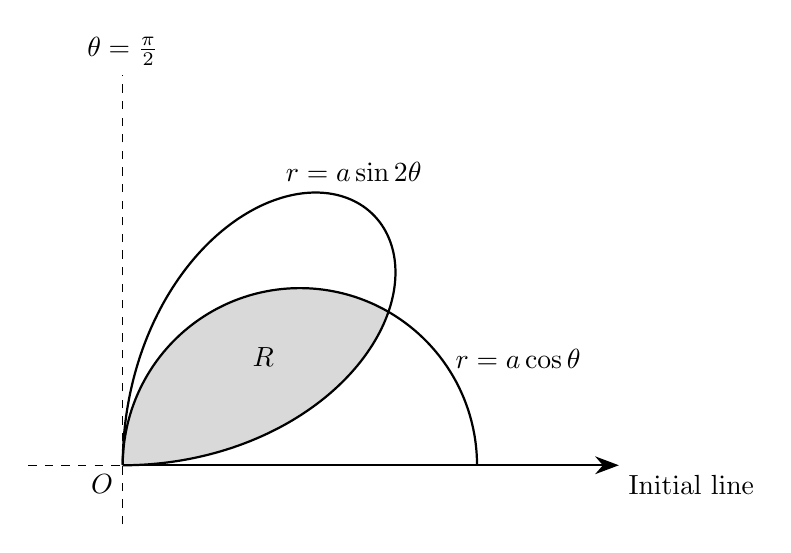
\begin{tikzpicture}[scale=1.5]
\def\a{3}
\pgfmathsetmacro{\thI}{pi/6}
\pgfmathsetmacro{\thMax}{pi/2}
\coordinate (O) at (0,0);
\coordinate (Xleft) at (-0.8,0);
\coordinate (Xend) at (4.2,0);
\coordinate (Ybot) at (0,-0.5);
\coordinate (Ytop) at (0,3.3);

\draw[dashed] (Xleft) -- (O);
\draw[-{Stealth[length=3mm]}, thick] (O) -- (Xend);
\draw[dashed] (Ybot) -- (Ytop);

\fill[gray!30]
  (O) --
  plot[smooth, samples=120, domain=0:\thI, variable=\t]
    ({\a*sin(2*deg(\t))*cos(deg(\t))},{\a*sin(2*deg(\t))*sin(deg(\t))})
  --
  plot[smooth, samples=120, domain=\thI:\thMax, variable=\t]
    ({\a*cos(deg(\t))*cos(deg(\t))},{\a*cos(deg(\t))*sin(deg(\t))})
  -- cycle;

\draw[thick, black]
  plot[smooth, samples=200, domain=0:\thMax, variable=\t]
    ({\a*sin(2*deg(\t))*cos(deg(\t))},{\a*sin(2*deg(\t))*sin(deg(\t))});

\draw[thick, black]
  plot[smooth, samples=200, domain=0:\thMax, variable=\t]
    ({\a*cos(deg(\t))*cos(deg(\t))},{\a*cos(deg(\t))*sin(deg(\t))});

\pgfmathsetmacro{\rR}{0.5*\a}
\coordinate (Rlab) at (37.5:\rR);
\pgfmathsetmacro{\thLabelRose}{pi/3}
\coordinate (Lrose) at ({\a*sin(2*deg(\thLabelRose))*cos(deg(\thLabelRose))},{\a*sin(2*deg(\thLabelRose))*sin(deg(\thLabelRose))});
\pgfmathsetmacro{\thLabelCircle}{pi/8}
\coordinate (Lcircle) at ({\a*cos(deg(\thLabelCircle))*cos(deg(\thLabelCircle))},{\a*cos(deg(\thLabelCircle))*sin(deg(\thLabelCircle))});

\node[below left] at (O) {$O$};
\node[below right] at (Xend) {Initial line};
\node[above] at (Ytop) {$\theta=\frac{\pi}{2}$};
\node at (Rlab) {$R$};
\node[above right, yshift=3pt] at (Lrose) {$r=a\sin 2\theta$};
\node[below right, xshift=7.5pt] at (Lcircle) {$r=a\cos\theta$};
\end{tikzpicture}
\end{figure}


In the first quadrant, the curve $r=a\sin 2\theta$ intersects the circle $r=a\cos\theta$ at the pole and at one other point. \\

The region $R$ shown consists of the points that lie inside both curves. \\

Find the exact area of $R$ in terms of $a$. \marks{8} \\

\newpage

% ---- Question 9 ----
\questionitem
% [Source: _QBT__Integration_of_Polar_Curves, Q9]

\begin{enumerate}[label=\textbf{(\alph*)}]
  \item On the same diagram, sketch the curve $C_1$ with polar equation
  \[
  r=2(1+\cos\theta),\quad 0\leq\theta\leq2\pi
  \]
  and the curve $C_2$ with polar equation $\theta=\frac{2\pi}{3}$. \marks{3} \\
  \item Find the area of the smaller region bounded by $C_1$ and $C_2$. \marks{6} \\
\end{enumerate}

\newpage

% ---- Question 10 ----
\questionitem
% [Source: _QBT__Integration_of_Polar_Curves, Q10]

\begin{figure}[H]
    \centering
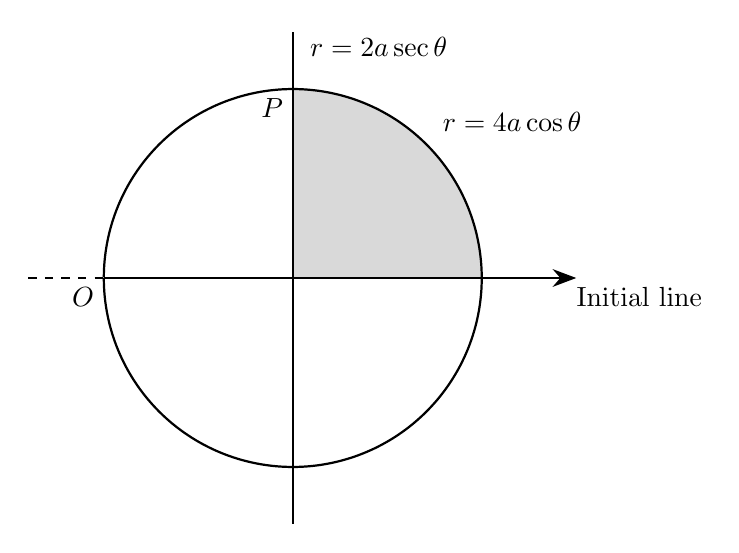
\begin{tikzpicture}[scale=1.2]
\def\a{1}
\def\th{0.785398} % pi/4

\coordinate (O) at (0,0);
\coordinate (A) at ({4*\a},0);
\coordinate (B) at ({2*\a},0);

\path[name path=circle]
  plot[smooth, samples=240, domain=-1.570796:1.570796]
    ({4*\a*cos(deg(\x))*cos(deg(\x))},
     {4*\a*cos(deg(\x))*sin(deg(\x))});
\path[name path=line] ({2*\a},{-2.6*\a}) -- ({2*\a},{2.6*\a});
\path[name intersections={of=circle and line, by={Q,P}}];

\fill[gray!30]
  (B) -- (P) --
  plot[smooth, samples=120, domain=\th:0]
    ({4*\a*cos(deg(\x))*cos(deg(\x))},
     {4*\a*cos(deg(\x))*sin(deg(\x))})
  -- cycle;

\draw[dashed, black] (-0.8,0) -- (0,0);
\draw[-{Stealth[length=3mm]}, thick, black] (0,0) -- (5,0);

\draw[thick, black]
  plot[smooth, samples=240, domain=-1.570796:1.570796]
    ({4*\a*cos(deg(\x))*cos(deg(\x))},
     {4*\a*cos(deg(\x))*sin(deg(\x))});
\draw[thick, black] ({2*\a},{-2.6*\a}) -- ({2*\a},{2.6*\a});

\node[below left] at (O) {$O$};
\node[below left] at (P) {$P$};
\node[below right] at (4.9,0) {Initial line};
\node[right] at ({2.08*\a},{2.45*\a}) {$r = 2a\sec\theta$};
\node[above, xshift=40pt] at ({3.15*\a},{1.45*\a}) {$r = 4a\cos\theta$};
\end{tikzpicture}
\end{figure}


The diagram shows a sketch of the curves with polar equations
\[
r=4a\cos\theta \text{ and } r=2a\sec\theta,\quad a>0
\] \\
\begin{enumerate}[label=\textbf{(\alph*)}]
  \item Find the polar coordinates of the point of intersection $P$ of the two curves in the first quadrant. \marks{4} \\
  \item Find the area, shaded in the figure, bounded by the two curves and by the initial line $\theta=0$, giving your answer in terms of $a$ and $\pi$. \marks{6} \\
\end{enumerate}

\newpage

% ---- Question 11 ----
\questionitem
% [Source: _QBT__Integration_of_Polar_Curves, Q11]

\begin{figure}[H]
    \centering
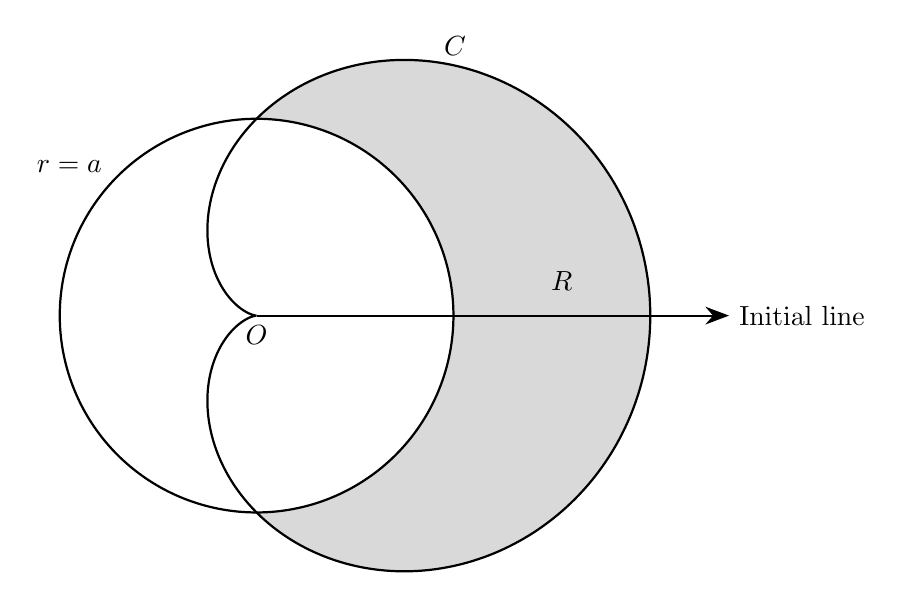
\begin{tikzpicture}[scale=1.25]
\def\a{2}
\coordinate (R) at ({1.55*\a},0.35);

\fill[gray!30]
  plot[smooth, samples=200, domain=-1.570796:1.570796, variable=\t]
    ({(\a*(1+cos(deg(\t))))*cos(deg(\t))},{(\a*(1+cos(deg(\t))))*sin(deg(\t))})
  --
  plot[smooth, samples=200, domain=1.570796:-1.570796, variable=\t]
    ({\a*cos(deg(\t))},{\a*sin(deg(\t))})
  -- cycle;

\pgfmathsetmacro{\tC}{0.9}
\draw[thick, black]
  plot[smooth, samples=300, domain=-pi:pi, variable=\t]
    ({(\a*(1+cos(deg(\t))))*cos(deg(\t))},
     {(\a*(1+cos(deg(\t))))*sin(deg(\t))});
\node[above] at
  ({(\a*(1+cos(deg(\tC))))*cos(deg(\tC))},
   {(\a*(1+cos(deg(\tC))))*sin(deg(\tC))}) {$C$};

\pgfmathsetmacro{\tr}{2.4}
\draw[thick, black]
  plot[smooth, samples=300, domain=0:2*pi, variable=\t]
    ({\a*cos(deg(\t))},
     {\a*sin(deg(\t))});
\node[above left] at
  ({\a*cos(deg(\tr))},
   {\a*sin(deg(\tr))}) {$r=a$};

\draw[-{Stealth[length=3mm]}, thick, black] (0,0) -- (4.8,0) node[right] {Initial line};
\node[below] at (0,0) {$O$};
\node at (R) {$R$};
\end{tikzpicture}
\end{figure}


The figure above shows a sketch of the curve $C$ with polar equation
\[
r=a(1+\cos\theta)
\] \\
and the circle
\[
r=a
\] \\
where $a>0$ and $-\pi\leq\theta\leq\pi$. \\

The shaded region inside $C$ and outside the circle has area
\[
18+\frac{9\pi}{4}
\] \\
Find the value of $a$. \marks{8} \\


\newpage

% ---- Question 12 ----
\questionitem
% [Source: _QBT__Integration_of_Polar_Curves, Q12]

\begin{figure}[H]
    \centering
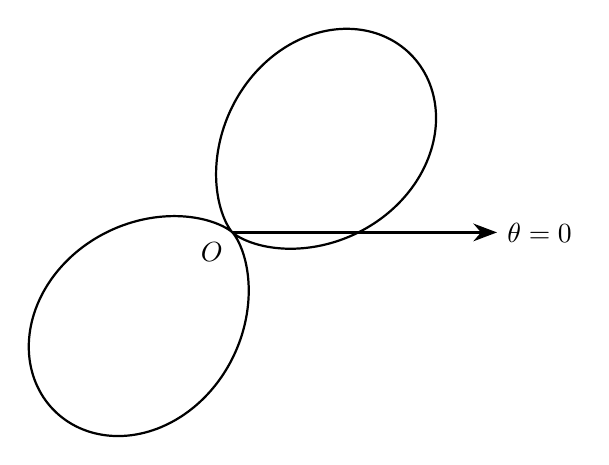
\begin{tikzpicture}[scale=1.6]
\def\twopi{6.283185}
\draw[-{Stealth[length=3mm]}, thick] (0,0) -- (2.1,0) node[right] {$\theta = 0$};
\draw[thick, black]
  plot[smooth, samples=400, domain=0:\twopi]
    ({(1+sin(deg(2*\x)))*cos(deg(\x))},{(1+sin(deg(2*\x)))*sin(deg(\x))});
\node[below left] at (0,0) {$O$};
\end{tikzpicture}
\end{figure}


The diagram below shows the curve with polar equation $r=1+\sin 2\theta$ for $0\leq\theta\leq2\pi$. \\
\begin{enumerate}[label=\textbf{(\alph*)}]
  \item Find the values of $\theta$ at the pole. \marks{1} \\
  \item Find the polar coordinates of the points on the curve where $r$ takes its maximum value. \marks{2} \\
  \item Find the exact total area enclosed by the curve. \marks{4} \\
  \item Find a Cartesian equation for the curve. \marks{2} \\
\end{enumerate}


\end{enumerate}
\end{document}
